% ============================================================
% 03-proposed-model.tex — CTU-Chat Proposed Architecture
% ============================================================
\section{Proposed Model}
\label{sec:model}

This section presents the architecture, algorithms, and evidence-acquisition mechanisms of \system{}. The proposed model is organized around three design principles: \emph{centralized agent coordination}, in which a supervisor dispatches each query to one domain agent without peer-to-peer delegation; \emph{heterogeneous knowledge allocation}, which assigns each information structure to a corresponding evidence representation; and \emph{representation-aware evidence routing}, which selects either a direct graph-tool path or an intent-scoped retrieval path according to the assigned domain. Here, each \emph{specialist} represents a bounded domain agent configured with dedicated prompt constraints, an assigned evidence store, and a restricted tool registry.

%------------------------------------------------
\subsection{Overall Proposed Architecture}
\label{sec:architecture}

Figure~\ref{fig:architecture} illustrates the system architecture of \system{}, structured across three coordinated tiers: (1)~the \emph{Interaction and Centralized Supervisor Tier}, (2)~the \emph{Domain-Specialized Multi-Agent Core Layer}, and (3)~the \emph{Heterogeneous Knowledge Storage and Tool Tier}.

\begin{figure}[!htbp]
\centering
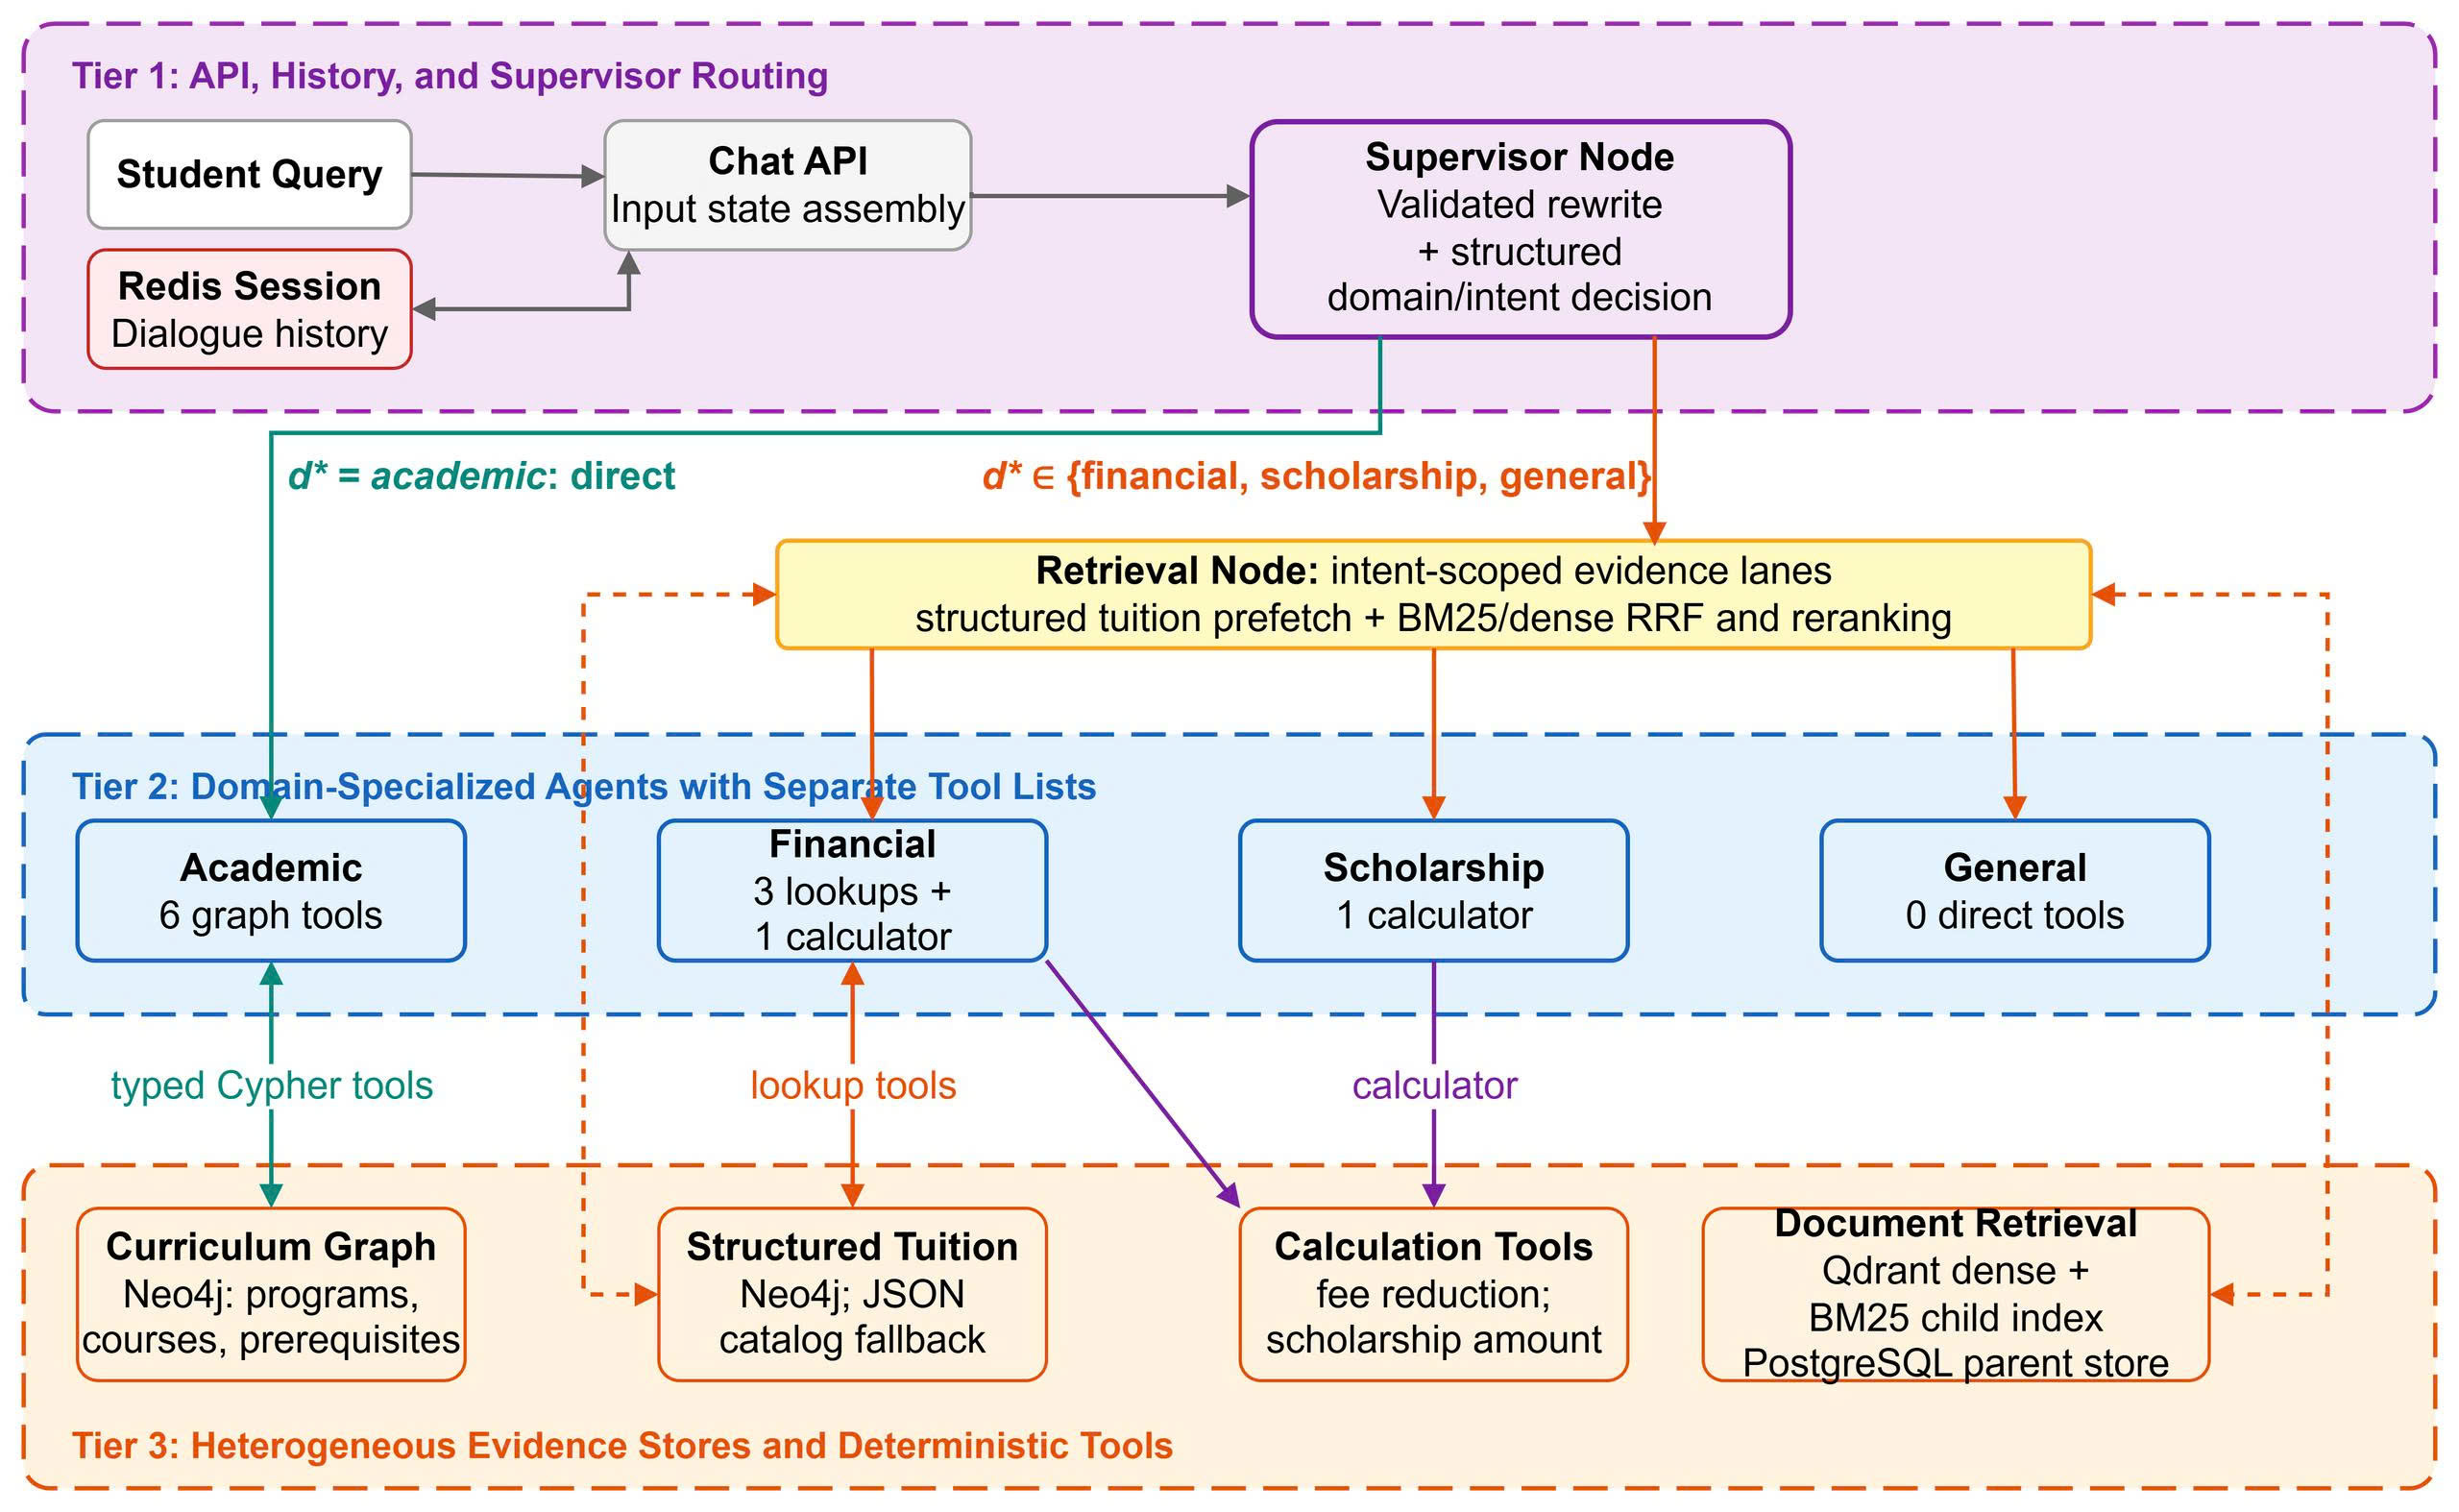
\includegraphics[width=\textwidth]{figures/architecture.jpg}
\caption{Implemented \system{} architecture. The Chat API loads dialogue history from Redis and supplies it in the graph input state. The first conditional edge sends academic queries directly to the graph-enabled agent and sends the other domains through intent-scoped retrieval; the second edge dispatches the retrieved evidence to the selected domain-specialized agent. Solid agent--resource links denote direct tool access, whereas dashed links denote evidence acquisition performed by the retrieval node.}
\label{fig:architecture}
\end{figure}
\FloatBarrier

\textbf{Application-Level Specialization of LangGraph StateGraph:}
Rather than modifying the underlying LangGraph engine, \system{} establishes an application-level orchestration policy governed by a typed state contract, isolated execution paths, and partitioned tool registries. Following supervisor dispatch, the four domain specialists operate independently without peer-to-peer delegation, selecting actions strictly from their construction-time tool bindings.
\begin{itemize}
    \setlength{\itemsep}{1.5pt}
    \setlength{\parsep}{0pt}
    \setlength{\parskip}{0pt}
    \item \textbf{Node-scoped state updates:} \texttt{AgentState} defines explicit write boundaries: the supervisor writes to the routing fields (\texttt{search\_query}, \texttt{next\_agent}, and \texttt{routing\_decision}); the retrieval node updates \texttt{context}; and each specialist returns \texttt{response}. This contract enforces transparent data ownership and mitigates cross-domain context pollution.
    
    \item \textbf{Two-Tier Conditional Routing Edges:} Instead of letting agents dynamically negotiate execution flow, the orchestration topology is governed by deterministic conditional functions:
    \begin{equation}
        \mathrm{Edge}_{\text{sup}}(\mathcal{S}) = \begin{cases}
            \text{'academic\_agent'}, & \text{if } \mathcal{S}[\text{'next\_agent'}] = \text{'academic'} \\
            \text{'retrieval'}, & \text{otherwise},
        \end{cases}
    \end{equation}
    bypassing document retrieval for queries assigned to the academic agent. At the retrieval exit, $\mathrm{Edge}_{\text{ret}}(\mathcal{S})$ dispatches the retrieved context to the selected financial, scholarship, or general agent.
    
    \item \textbf{Acyclic outer orchestration:} The StateGraph has no peer-to-peer agent edges. Each selected domain-specialized agent returns to \texttt{END}, so the outer routing path cannot cycle. ReAct tool interactions inside an agent remain distinct from this outer graph topology.
    
    \item \textbf{Domain-specialized agents with asymmetric tools:} The academic, financial, and scholarship agents are constructed with separate prompts and tool lists, while the general agent has no direct tool (as detailed in Figure~\ref{fig:architecture}). This confines tool selection to the agent selected by the supervisor and keeps domain-specific evidence paths separate, reducing decision space pollution.
\end{itemize}

%------------------------------------------------
\subsection{Neo4j Knowledge Graph Specification and Cypher Tool Mechanics}
\label{sec:neo4j_graph}

\textbf{Schema defined by the ingestion layer:}
The Neo4j graph models relational dependencies across academic counseling without ontological overhead, comprising over 1,500 entity nodes and 3,800 relational edges across 113 undergraduate curricula and statutory fee schedules. It incorporates 10 node labels (7 for curriculum: \texttt{Program}, \texttt{Course}, \texttt{Block}, etc.; and 3 for tuition: \texttt{TuitionFee}, \texttt{TuitionPolicy}, \texttt{ExemptionBasisRate}) interconnected via 13 relationship types (\texttt{HAS\_BLOCK}, \texttt{CONTAINS}, \texttt{REQUIRES}, \texttt{PARALLEL\_WITH}, \texttt{HAS\_PLO}, \texttt{HAS\_PEO}, \texttt{REALIZED\_BY}, \texttt{HAS\_TRACK}, \texttt{BELONGS\_TO\_TRACK}, \texttt{HAS\_JOB\_POSITION}, \texttt{HAS\_TUITION}, \texttt{GOVERNED\_BY}, and \texttt{HAS\_EXEMPTION\_BASIS}). Narrative regulations remain in the document store unless linked to structured entities.

\textbf{Cypher tool mechanics:}
The system does not ask the LLM to generate arbitrary Cypher. After the supervisor selects the academic agent, its ReAct policy chooses one of six typed tools and supplies the tool arguments. The tool normalizes identifiers or names and calls a fixed, parameterized Cypher query in the graph service. The tools implement three query classes:
\begin{itemize}
    \setlength{\itemsep}{1.5pt}
    \setlength{\parsep}{0pt}
    \setlength{\parskip}{0pt}
    \item \emph{Attribute lookup and search}: \texttt{tra\_cuu\_nganh} and \texttt{tim\_nganh} match program codes or normalized program, unit, and course names; \texttt{so\_sanh\_nganh} applies the same lookup before comparing two programs.
    \item \emph{Structural traversal}: \texttt{xem\_chuoi\_tien\_quyet} follows \texttt{REQUIRES} paths up to ten hops and returns direct \texttt{PARALLEL\_WITH} courses. \texttt{mon\_chung\_giua\_nganh} computes a course intersection across two program--block paths, and \texttt{tim\_nganh\_co\_mon} traverses those paths in reverse.
    \item \emph{Structured financial lookup}: parameterized queries match \texttt{TuitionFee}, \texttt{TuitionPolicy}, and \texttt{ExemptionBasisRate} properties and their program relationships. This graph lookup is separate from the BM25--dense hybrid document retrieval path used for narrative regulations.
\end{itemize}
This design binds agent actions directly to deterministic graph operations: the LLM only selects the appropriate tool and supplies its arguments, while the query topology remains fixed and parameterized within the graph service. As a result, the multi-agent workflow reliably incorporates graph evidence while mitigating the syntactic and semantic fragility typically associated with unconstrained Cypher generation.

%------------------------------------------------
\subsection{Algorithmic Foundations: Routing and Deterministic Arithmetic}
\label{sec:algorithms}

Algorithm~\ref{alg:routing} specifies the supervisor-routing and evidence-path dispatch procedure.

\begin{algorithm}[!htbp]
\footnotesize
\SetAlFnt{\footnotesize}
\SetAlCapFnt{\footnotesize}
\SetAlCapNameFnt{\footnotesize}
\SetAlgoVlined
\LinesNumbered
\caption{Supervisor Routing and Conditional Evidence-Path Dispatch}
\label{alg:routing}
\KwIn{Student query $q$, Dialogue history $\mathcal{H}$, Shared state $\mathcal{S}$}
\KwOut{State updates and next graph node}
$q_{\text{standalone}} \leftarrow q$\;
$q_{\mathrm{prev}} \leftarrow \mathrm{MostRecentUserQuery}(\mathcal{H})$\;
\If{$\mathrm{ShouldRewriteQuery}(q, q_{\mathrm{prev}})$}{
    $q_{\text{cand}} \leftarrow \mathrm{FastLLM\_Rewrite}(q, q_{\mathrm{prev}})$\;
    \If{$\mathrm{ValidateRewrite}(q, q_{\text{cand}}, q_{\mathrm{prev}})$}{
        $q_{\text{standalone}} \leftarrow q_{\text{cand}}$\;
    }
}
$\langle d^*, \iota^* \rangle \leftarrow \mathrm{StructuredSupervisor}(q)$\;
\If{structured classification fails}{
    $d^* \leftarrow \text{'general'}$; $\iota^* \leftarrow \text{'other'}$\;
}
Update $\mathcal{S}[\texttt{search\_query}] \leftarrow q_{\text{standalone}}$, $\mathcal{S}[\texttt{next\_agent}] \leftarrow d^*$, and $\mathcal{S}[\texttt{routing\_decision}] \leftarrow \mathrm{QueryRoutingDecision}(\iota^*)$\;
\eIf{$d^* = \text{'academic'}$}{
    $v_{\text{next}} \leftarrow \text{'academic\_agent'}$\;
}{
    Build retrieval lanes from $\iota^*$ and retrieve evidence\;
    $v_{\text{next}} \leftarrow d^*\texttt{\_agent}$\;
}
\Return $\langle \mathcal{S}, v_{\text{next}} \rangle$\;
\end{algorithm}

A candidate rewrite is adopted only after validation; structured output restricts classification to declared labels with \texttt{general}/\texttt{other} as fallback; and conditional edges route academic queries directly to the agent while other domains pass through retrieval.

\textbf{Deterministic Tuition Reduction Arithmetic:}
For fee-reduction requests, \system{} augments the LLM with the external deterministic tool \texttt{tinh\_toan\_hoc\_phi}. The LLM interprets the request and supplies three parameters---the actual per-credit tuition $T$, the per-credit exemption basis $B$, and the percentage entitlement $p$---but does not perform the arithmetic through free-form text generation. The external tool validates the percentage range and applies the fixed calculation
\begin{equation}
  D = B\frac{p}{100}, \qquad P = \max(0, T-D).
  \label{eq:tuition_reduction}
\end{equation}
where $D$ is the reduction per credit and $P$ is the remaining amount per credit. Monetary inputs are expected in VND per credit. The tool enforces $0 \le p \le 100$ and clamps $P$ at zero; values outside the percentage range return an error.

Rather than a new general-purpose algorithm, the contribution lies in composing validated rewriting, constrained routing, representation-specific dispatch, and deterministic arithmetic within the multi-agent workflow.

%------------------------------------------------
\subsection{Heterogeneous Knowledge Allocation and Hybrid Retrieval}
\label{sec:hybrid_retrieval}

This layer implements \emph{heterogeneous knowledge allocation}: rather than forcing all institutional knowledge into a uniform document index, \system{} preserves relational curriculum knowledge in Neo4j, accesses cohort-dependent tuition data through structured lookup, and retains narrative regulations and scholarship policies in document retrieval.

Table~\ref{tab:decision_criteria} makes this policy explicit by separating the physical evidence representation from the mechanism used to access it at runtime.

\begin{table}[h!]
\centering
\caption{Decision criteria mapping query characteristics to evidence representation mechanisms.}
\label{tab:decision_criteria}
\setlength{\tabcolsep}{3pt}
\renewcommand{\arraystretch}{1.1}
\begin{tabular}{>{\raggedright\arraybackslash}p{0.30\columnwidth}>{\raggedright\arraybackslash}p{0.29\columnwidth}>{\raggedright\arraybackslash}p{0.30\columnwidth}}
\toprule
\textbf{Query characteristic} & \textbf{Evidence path} & \textbf{Rationale} \\
\midrule
Program/course attributes & Neo4j property lookup & Exact or normalized match \\
Prerequisites/shared courses & Neo4j traversal & Stored graph relationships \\
Regulation identifiers & BM25 child index & Exact token match \\
Paraphrased regulations & Hybrid RRF + reranker & Lexical + semantic signals \\
Fee/scholarship calculation & Python tool & Fixed formula outside LLM \\
\bottomrule
\end{tabular}
\end{table}

At runtime, the StateGraph enforces this allocation. Academic queries bypass the document-retrieval node and enter the graph-enabled academic agent directly. Financial, scholarship, and general queries enter the retrieval node, where the supervisor-assigned intent selects metadata-filtered retrieval lanes before the resulting context is passed only to the assigned domain agent.

\textbf{Hybrid Document Retrieval Path.}
For narrative regulations and scholarship criteria, evidence is acquired
through the following pipeline:

\begin{enumerate}
    \setlength{\itemsep}{1.5pt}
    \setlength{\parsep}{0pt}
    \setlength{\parskip}{0pt}
    \item \emph{Child-level candidate generation.}
    A BM25 index searches child chunks, while Qdrant performs dense retrieval
    over their 768-dimensional embeddings.

    \item \emph{Parent resolution.}
    Parent identifiers associated with the retrieved child chunks are used to
    load the corresponding parent sections from PostgreSQL.

    \item \emph{Reciprocal Rank Fusion.}
    The dense- and BM25-derived parent rankings are combined as
    \[
        s_{\mathrm{RRF}}(d)
        = \sum_{s\in\{\mathrm{bm25},\mathrm{dense}\}}
          \frac{1}{k+r_s(d)}, \qquad k=60.
    \]

    \item \emph{Cross-encoder reranking.}
    The fused parent candidates are reranked using
    \texttt{BAAI/bge-reranker-v2-m3}, and up to six parent sections are
    supplied to the selected domain agent.
\end{enumerate}

Parent sections use a 2,800-character target with 100-character overlap;
child chunks use a 400-character target with 50-character overlap.
